%%%%%%%%%%%%%%%%%%%%%%%%%%%%%%%%%%%%%%%%%
% Short Sectioned Assignment
% LaTeX Template
% Version 1.0 (5/5/12)
%
% This template has been downloaded from:
% http://www.LaTeXTemplates.com
%
% Original author:
% Frits Wenneker (http://www.howtotex.com)
%
% License:
% CC BY-NC-SA 3.0 (http://creativecommons.org/licenses/by-nc-sa/3.0/)
%
%%%%%%%%%%%%%%%%%%%%%%%%%%%%%%%%%%%%%%%%%

%----------------------------------------------------------------------------------------
%	PACKAGES AND OTHER DOCUMENT CONFIGURATIONS
%----------------------------------------------------------------------------------------

\documentclass[paper=a4, fontsize=11pt]{scrartcl} % A4 paper and 11pt font size

\usepackage[T1]{fontenc} % Use 8-bit encoding that has 256 glyphs
\usepackage{fourier} % Use the Adobe Utopia font for the document - comment this line to return to the LaTeX default
\usepackage[english]{babel} % English language/hyphenation

\usepackage{lipsum} % Used for inserting dummy 'Lorem ipsum' text into the template

\usepackage{sectsty} % Allows customizing section commands
\allsectionsfont{ \normalfont\scshape} % Make all sections centered, the default font and small caps
\usepackage{cite}
\usepackage{listings}

%%%%%---------------------------%%%%%%%%%%%
\usepackage{fancybox}
\usepackage{graphicx}
\usepackage{pdfpages}
\usepackage{color}
\usepackage{epstopdf}
\usepackage[margin=1in, vmargin=1in]{geometry}
\usepackage{mathtools}
\usepackage{float}
\usepackage{listings}
\usepackage{verbatim}
\usepackage{booktabs}
\usepackage{tabularx}
\usepackage{longtable}
\usepackage{movie15}
\usepackage{hyperref}
\usepackage{subcaption}
\usepackage{enumerate}
\usepackage{hyperref}
\usepackage{bashful}

\usepackage{multicol}
%%%%%%%%%%%%%%---------------%%%%%%%%


\usepackage{fancyhdr} % Custom headers and footers
\pagestyle{fancyplain} % Makes all pages in the document conform to the custom headers and footers
\fancyhead{} % No page header - if you want one, create it in the same way as the footers below
\fancyfoot[L]{} % Empty left footer
\fancyfoot[C]{} % Empty center footer
\fancyfoot[R]{\thepage} % Page numbering for right footer
\renewcommand{\headrulewidth}{0pt} % Remove header underlines
\renewcommand{\footrulewidth}{0pt} % Remove footer underlines
\setlength{\headheight}{13.6pt} % Customize the height of the header

\numberwithin{equation}{section} % Number equations within sections (i.e. 1.1, 1.2, 2.1, 2.2 instead of 1, 2, 3, 4)
\numberwithin{figure}{section} % Number figures within sections (i.e. 1.1, 1.2, 2.1, 2.2 instead of 1, 2, 3, 4)
\numberwithin{table}{section} % Number tables within sections (i.e. 1.1, 1.2, 2.1, 2.2 instead of 1, 2, 3, 4)

\setlength\parindent{0pt} % Removes all indentation from paragraphs - comment this line for an assignment with lots of text

%%%%%%%%CODE INPUT STYLES%%%%%%%%%%%%%
\lstdefinestyle{BashInputStyle}{
  language=bash,
  firstline=2,% Supress the first line that begins with `%`
  basicstyle=\small\sffamily,
  numbers=left,
  numberstyle=\tiny,
  numbersep=3pt,
  frame=tb,
  columns=fullflexible,
  backgroundcolor=\color{yellow!20},
  linewidth=0.9\linewidth,
  xleftmargin=0.1\linewidth
}

\lstdefinestyle{BashOutputStyle}{
  basicstyle=\small\ttfamily,
  numbers=none,
  frame=tblr,
  columns=fullflexible,
  backgroundcolor=\color{blue!10},
  linewidth=0.9\linewidth,
  xleftmargin=0.1\linewidth
}


% settings for listings
\lstset{
    basicstyle=\scriptsize,
    numbers=left,
    numberstyle=\scriptsize,
    stepnumber=1,
    numbersep=5pt,
    showspaces=false, % don't show spaces by adding underscores
    showstringspaces=false, % don't underline spaces in strings
    showtabs=false, % don't show tabs with underscores
    frame=shadowbox,
    tabsize=4,
    captionpos=b,
    breaklines=true,
    breakatwhitespace=false,
    keywordstyle=\color{blue!70},
    commentstyle=\color{red!50!green!50!blue!50},
    rulesepcolor=\color{red!20!green!20!blue!20},
    numberbychapter=false,
    stringstyle=\ttfamily %typewriter type for strings
}
\hypersetup{
colorlinks=true,
linkcolor=black,
citecolor=black,
urlcolor=black
}

%----------------------------------------------------------------------------------------
%	TITLE SECTION
%----------------------------------------------------------------------------------------

\newcommand{\horrule}[1]{\rule{\linewidth}{#1}} % Create horizontal rule command with 1 argument of height

\title{	
\normalfont \normalsize 
\textsc{Introduction to Web Science- Fall 2014} \\ [25pt] % Your university, school and/or department name(s)
\horrule{0.5pt} \\[0.4cm] % Thin top horizontal rule
\huge Assignment Six \\ % The assignment title
\horrule{2pt} \\[0.5cm] % Thick bottom horizontal rule
}

\author{Sybil Melton} % Your name

\date{\normalsize\today} % Today's date or a custom date

\begin{document}

\maketitle % Print the title
\newpage
\tableofcontents
\listoffigures
%\listoftables
\lstlistoflistings
\newpage
%----------------------------------------------------------------------------------------
%	TASK 1
%----------------------------------------------------------------------------------------

\section{Karate Club Split into Two}

We know the result of the Karate Club (Zachary, 1977) split.
Prove or disprove that the result of split could have been predicted
by the weighted graph of social interactions.  How well does the
mathematical model represent reality?

\subsection{Solution}
This problem was approached by learning the NetworkX graph programming.
The given data, a matrix of individuals and their connection strength to each other, was saved as a CSV file\cite{bib:zach-data}.
Row and column one, designates Mr. Hi and 34 designates John A., the two faction leaders.\cite{bib:zach-paper}
The python csv reader read each line as string list, which resulted in a list of lists and made it easier to parse into a list of weighted edges.\cite{bib:csv}
If the weight was greater than 0, it was added to the edge list as a tuple of individual, connected individual, and weight.
Then a weighted NetworkX graph was created by adding the weighted edge list.
The original Karate Club graph was saved as a dot file using Pydot, and used to create Figure \ref{fig:karateclub} using Gephi.\cite{bib:nx-tut}

\begin{figure}[H]
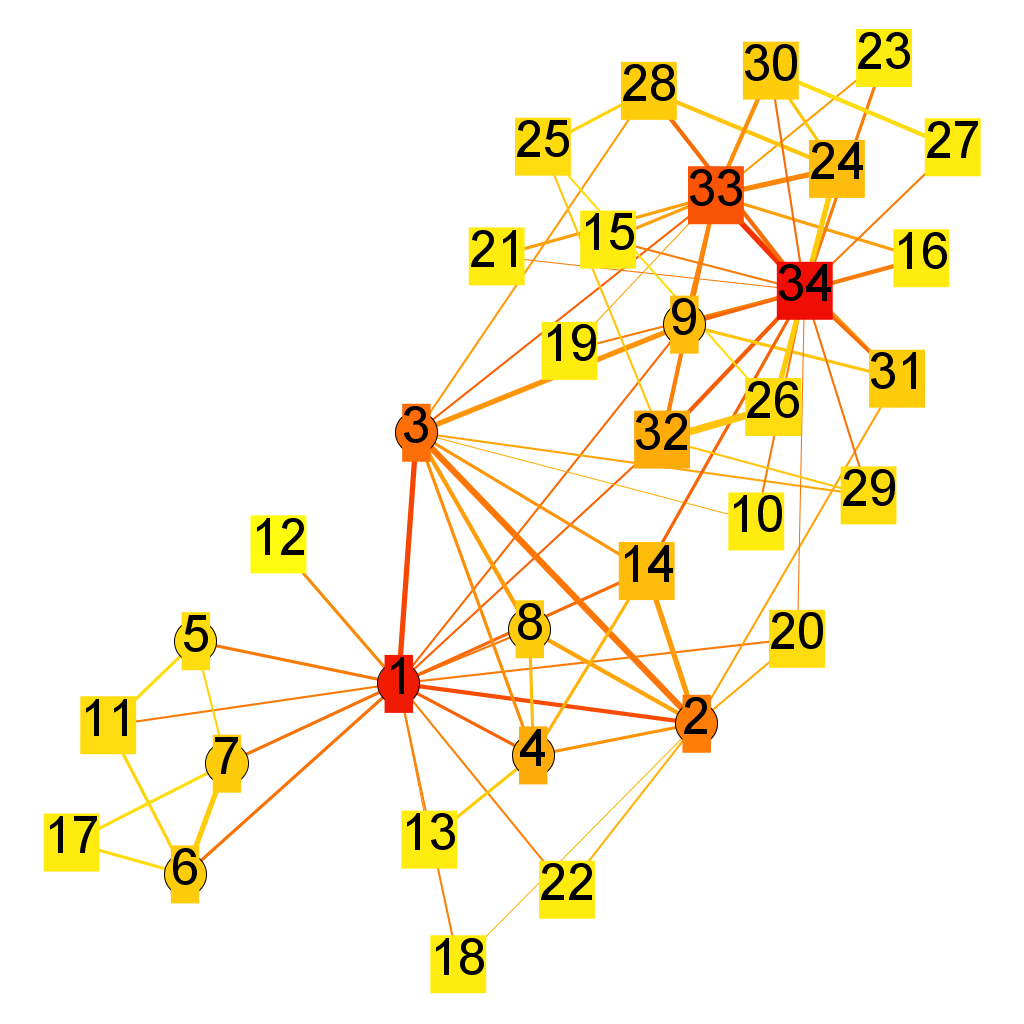
\includegraphics[width=1\textwidth]{weighted/karateclub}
\caption{Original Karate Club}
\label{fig:karateclub}
\end{figure}

NetworkX has the ability to create subgraphs by grouping the connected components together.
The result is a subgraph list.\cite{bib:subgraph} 
Using \emph{edge  betweenness} and the algorithm of Girvan and Newman, the Karate Club graph was split into two.
The steps of the algorithm are:
\begin{enumerate}
\item Compute edge centrality.
\item Remove edge with largest centrality, choose randomly for a tie.
\item  Recalculate edge centralities on the running graph.
\item Repeat from step 2.\cite{bib:community}
\end{enumerate}

``Betweenness centrality of an edge e is the sum of the fraction of all-pairs shortest paths that pass through e:
\[ \sum_{x,t\in V} \frac{\sigma(s,t|e)} {\sigma(s,t)}\]
where \(V\) is the set of nodes, \(\sigma(s, t)\) is the number of shortest \((s, t)\)-paths, and \(\sigma(s, t|e)\) is the number of those paths passing through edge e.''\cite{bib:edge-btn}
A loop kept track of the length of the subgraph list and terminated when it reach two.
Each iteration recalculated the edge betweenness centrality.
It kept a running list of the removed edges and printed them out upon completion with sorted node lists for each subgraph.
Figure \ref{fig:output} shows the output upon completion of creating the 2 subgraphs.

\begin{figure}[H]
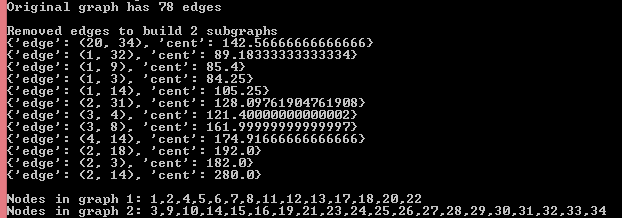
\includegraphics[width=1\textwidth]{weighted/output}
\caption{Program Output 2 Clubs}
\label{fig:output}
\end{figure}

The resulting subgraphs were also saved as dot files, in order to create Figures \ref{fig:club1} and \ref{fig:club2}.

\begin{figure}[H]
\centering
\begin{minipage}{.5\textwidth}
  \centering
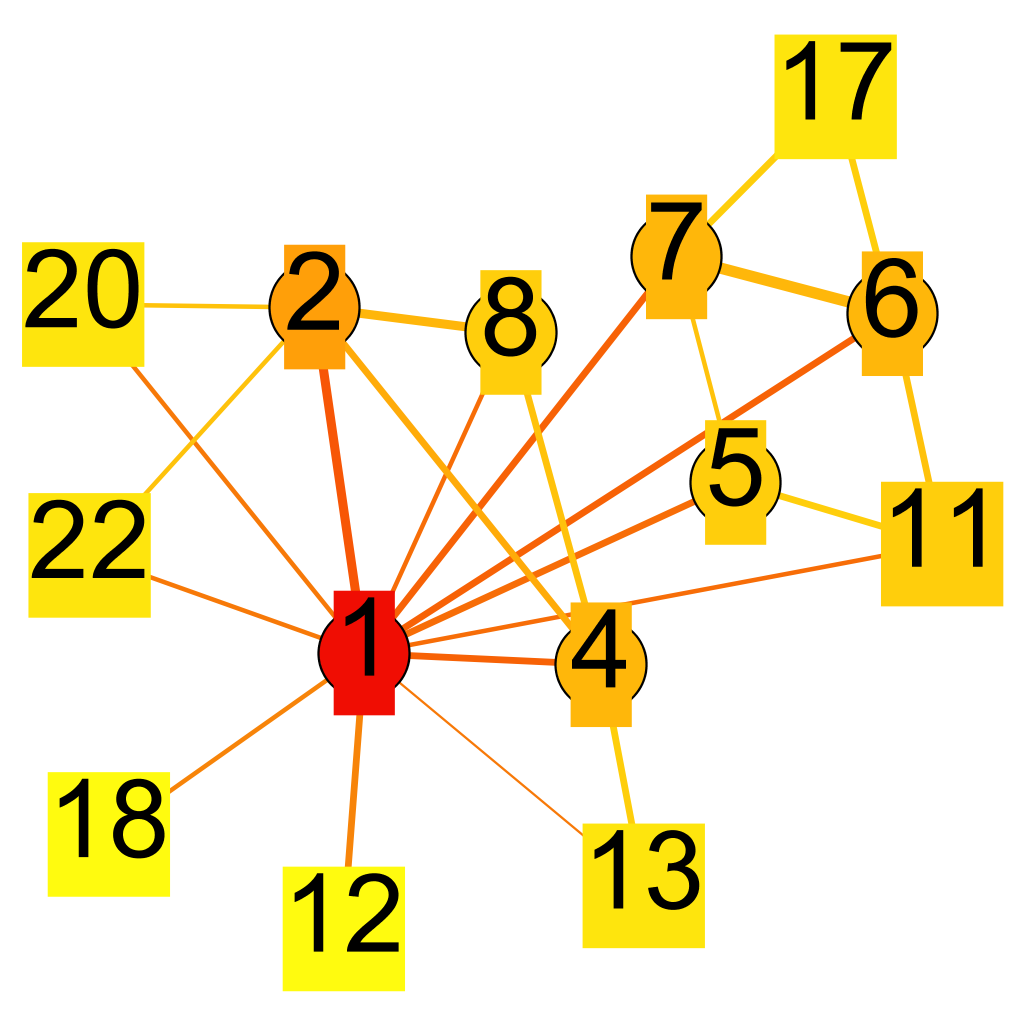
\includegraphics[width=1\textwidth]{weighted/club1}
\caption{2-way Split Club 1}
\label{fig:club1}
\end{minipage}%
\begin{minipage}{.5\textwidth}
  \centering
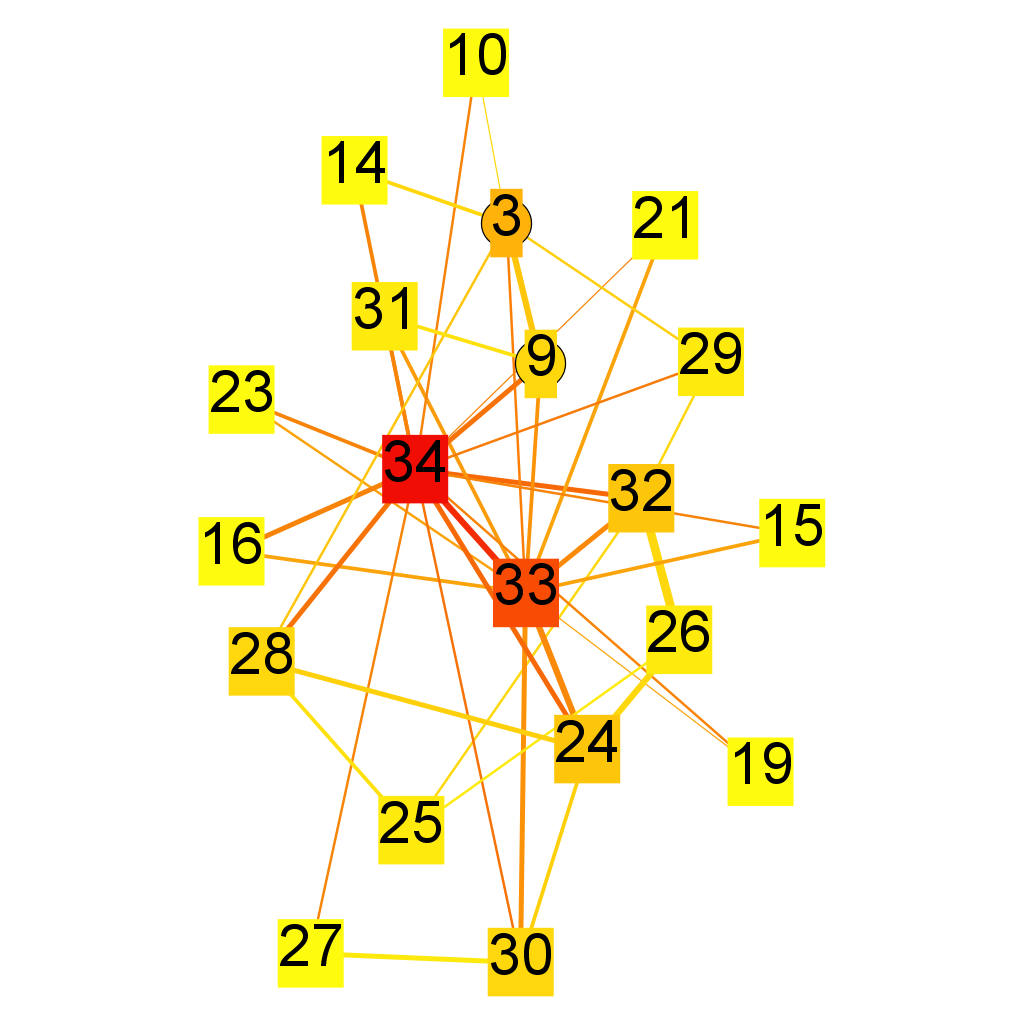
\includegraphics[width=1\textwidth]{weighted/club2}
\caption{2-way Split Club 2}
\label{fig:club2}
\end{minipage}
\end{figure}

The entire python program is included in Section \ref{sec:graph-code}, in Listing \ref{code:graphs}.
The code for calculating edge betweenness centrality, including the shortest path algorithm is included with this report as betweenness.py.
The connected component subgraph code is included in connected.py. 
Both files are unedited versions from the Pythonxy distribution.

\subsection{Result}

In my result, there were three individuals; 3, 9, and 14; who should have been in the graph with Mr. Hi (individual 1).
Mathematical models using only edge betweenness cannot always be 100\% correct.  
For example, individual nine had joined Mr. Hi's club, although he supported John A., for reasons unrelated to the split.\cite{bib:zach-paper}
In order to deduce a reason three and 14 ended up in the wrong graph, I looked at their positions in the original club.
Both were individuals had ties to both sides, so as more edges were removed, their edge betweenness centrality increased.
I believe the edge weights kept their edge betweenness centrality higher eventually led to being disconnected from Mr. Hi's graph.
Perhaps if the strength of their ties to Mr. Hi's supporters had also been taken into account, it would have resulted closer to reality.
The rest of the individuals were placed into the correct graph, so the Girvan and Newman algorithm was over 91\% correct.

\newpage
\subsection{Python Code}
\label{sec:graph-code}
%%% Code Listing%%%%%

\lstset{
    language=python,
    caption={Python graph code},
     label=code:graphs
}

\lstinputlisting{graphs.py}
\newpage 
%----------------------------------------------------------------------------------------
%           TASK 2
%----------------------------------------------------------------------------------------

\section{Karate Club Multiple Splits}
We know the group split in two different groups.  Suppose the
disagreements in the group were more nuanced -- what would the clubs
look like if they split into groups of 3, 4, and 5?

\subsection{Result}
The graphs program was written with the desired number of subgraphs as an argument.
The loop kept removing edges until the graph was split into the desired number of subgraphs.
The resulting dot files are included with this report and were used to create the resulting graphs.
As the group split into more subgroups, the next subgroup split from one of the two larger subgroups.
So the third group in the 4- and 5-way splits remained, as well as the fourth group remained in the 5-way split.
The screen output and each resulting graph are illustrated in the following sections.

\subsubsection{Three Clubs}
\begin{figure}[H]
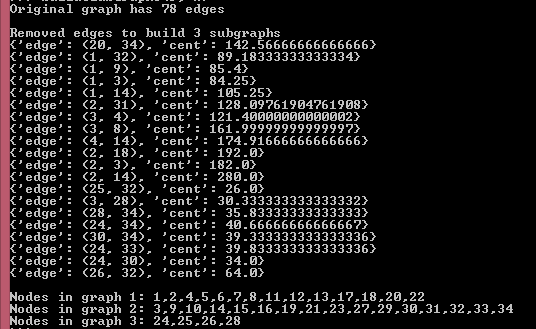
\includegraphics[width=1\textwidth]{3clubs/output}
\caption{Program Output 3 Clubs}
\label{fig:output3}
\end{figure}

\begin{figure}[H]
\centering
\begin{minipage}{.3\textwidth}
  \centering
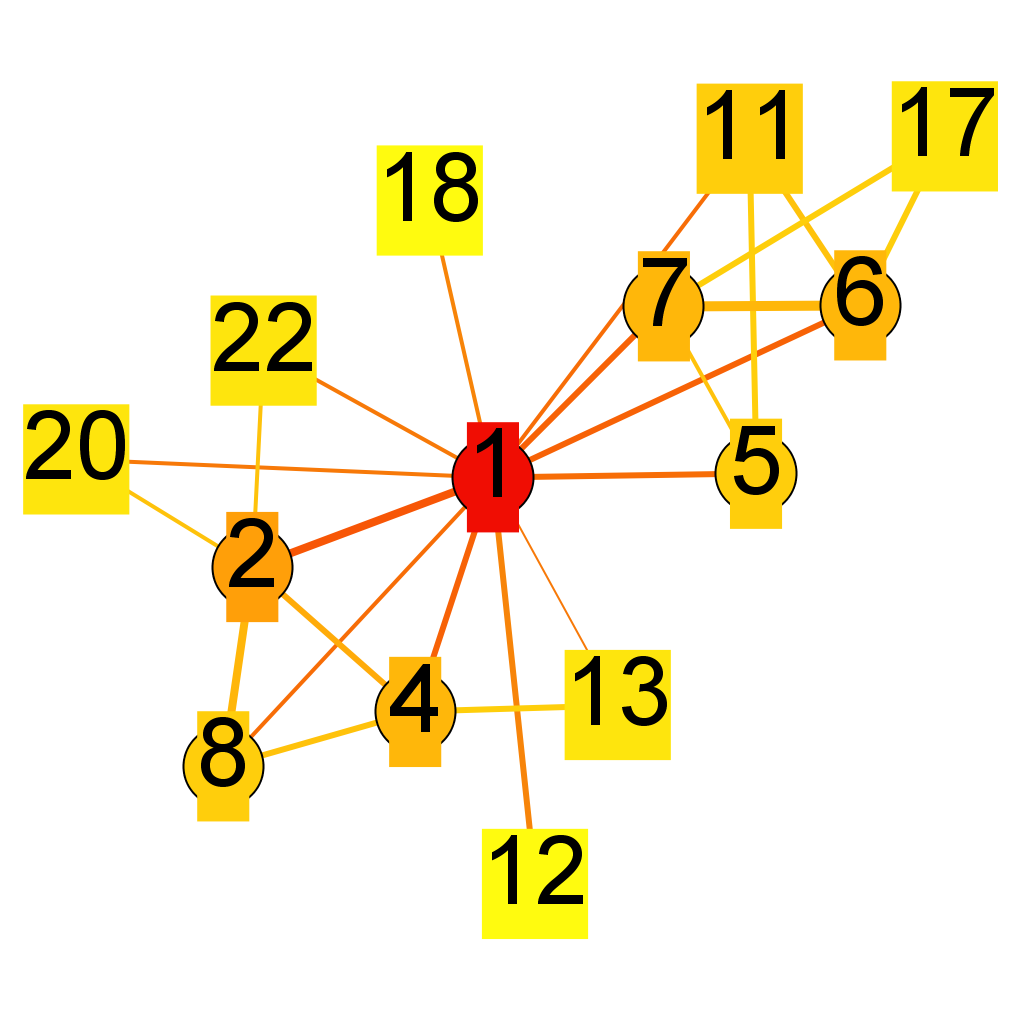
\includegraphics[width=1\textwidth]{3clubs/club1}
\caption{3-way Split Club 1}
\label{fig:3clubs1}
\end{minipage}%
\begin{minipage}{.4\textwidth}
  \centering
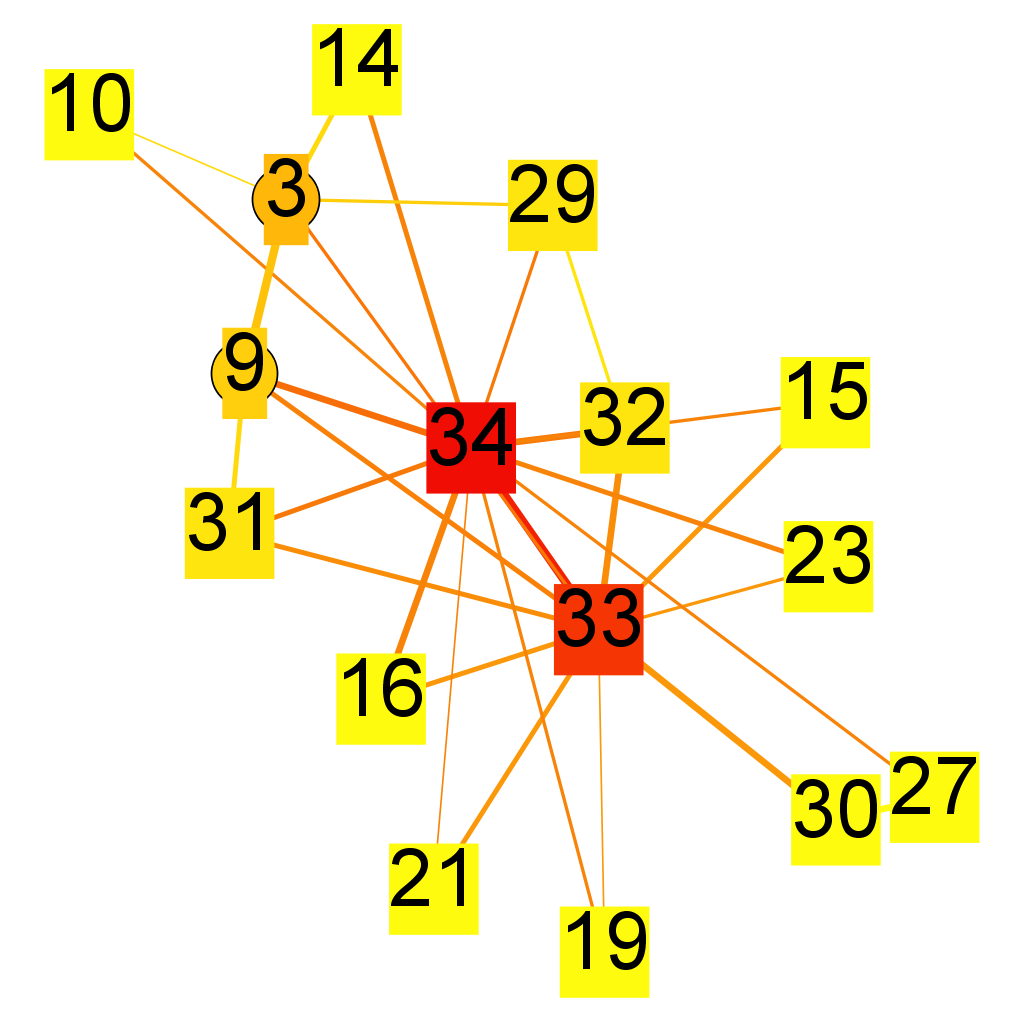
\includegraphics[width=1\textwidth]{3clubs/club2}
\caption{3-way Split Club 2}
\label{fig:3clubs2}
\end{minipage}%
\begin{minipage}{.25\textwidth}
  \centering
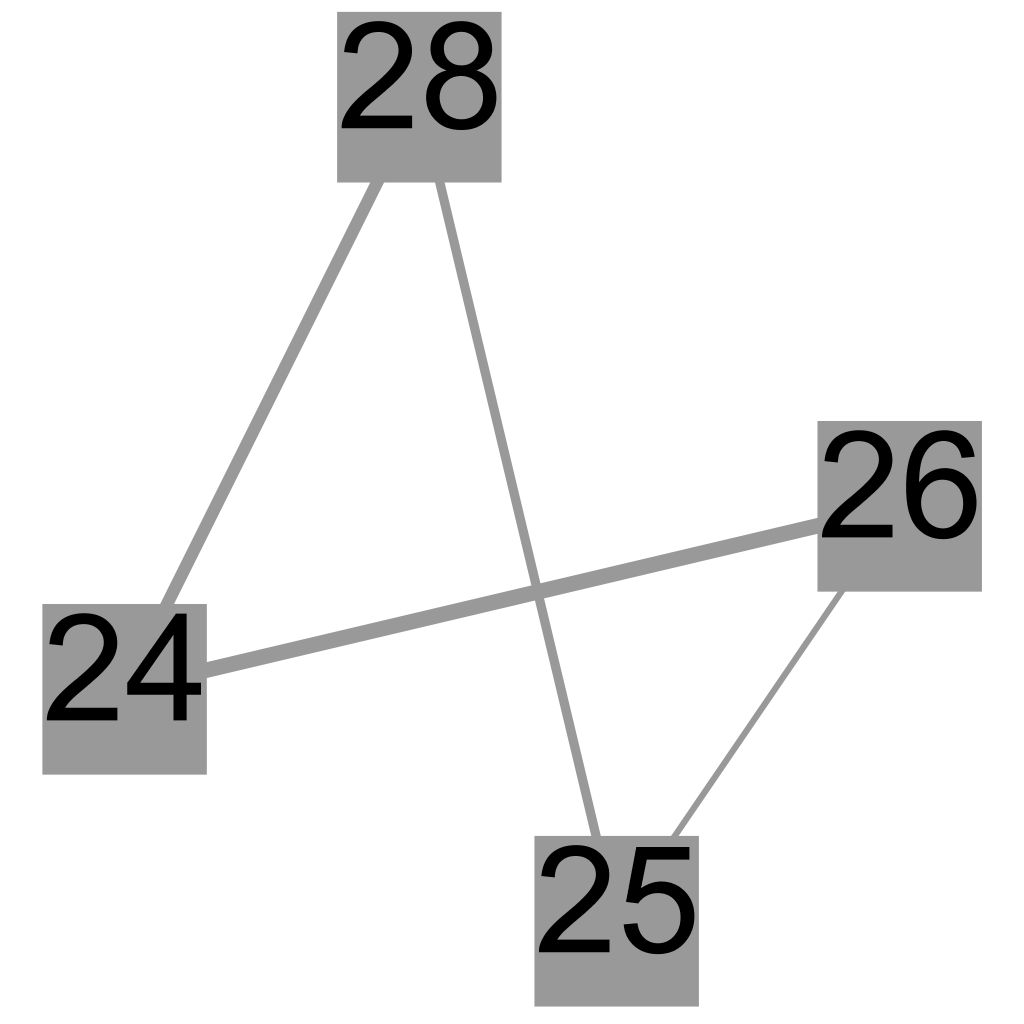
\includegraphics[width=1\textwidth]{3clubs/club3}
\caption{3-way Split Club 3}
\label{fig:3clubs3}
\end{minipage}
\end{figure}

\subsubsection{Four Clubs}
\begin{figure}[H]
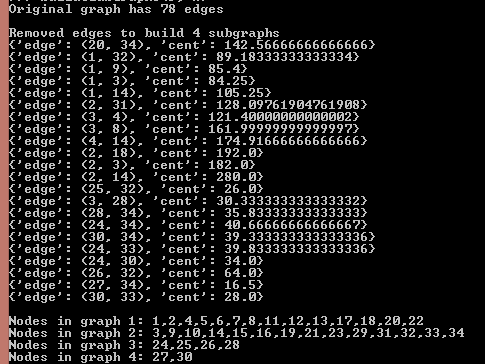
\includegraphics[width=1\textwidth]{4clubs/output}
\caption{Program Output 4 Clubs}
\label{fig:output4}
\end{figure}

\begin{figure}[H]
\centering
\begin{minipage}{.5\textwidth}
  \centering
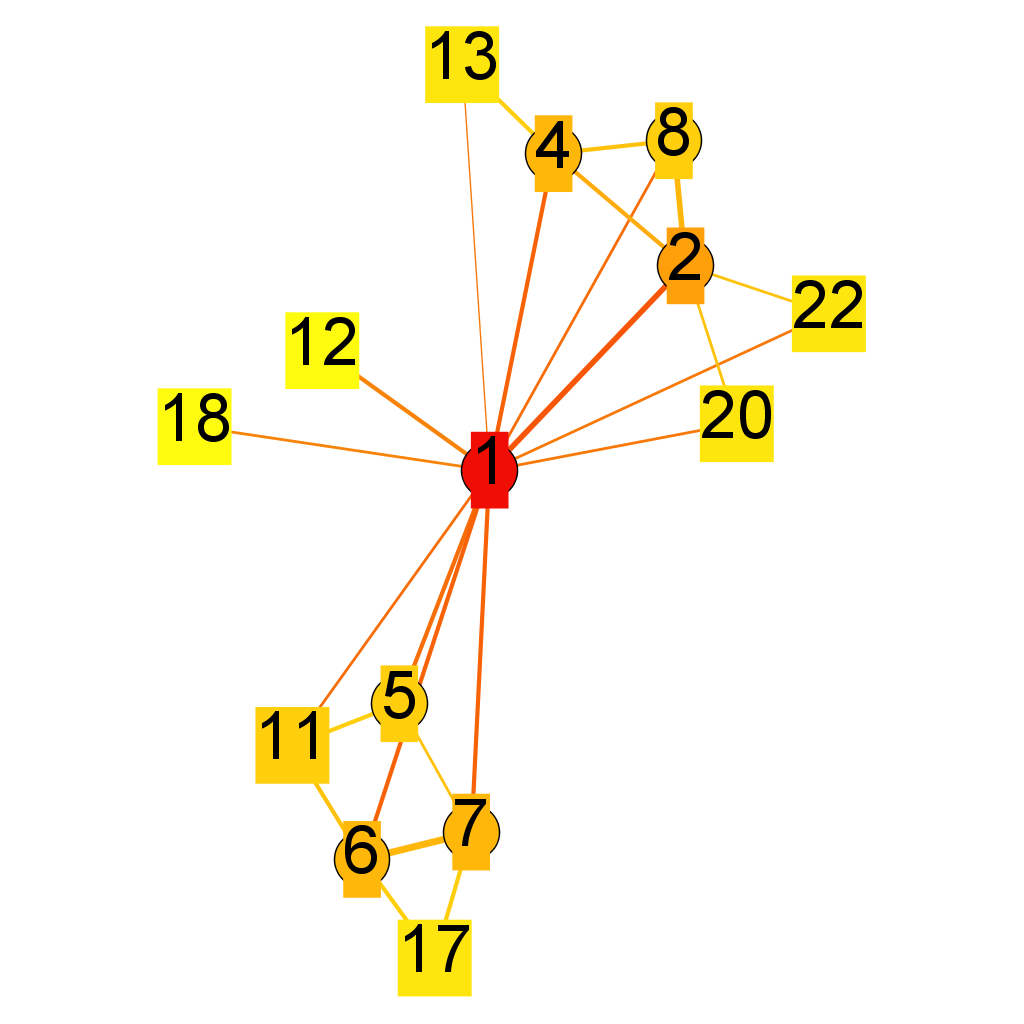
\includegraphics[width=1\textwidth]{4clubs/club1}
\caption{4-way Split Club 1}
\label{fig:4clubs1}
\end{minipage}%
\begin{minipage}{.5\textwidth}
  \centering
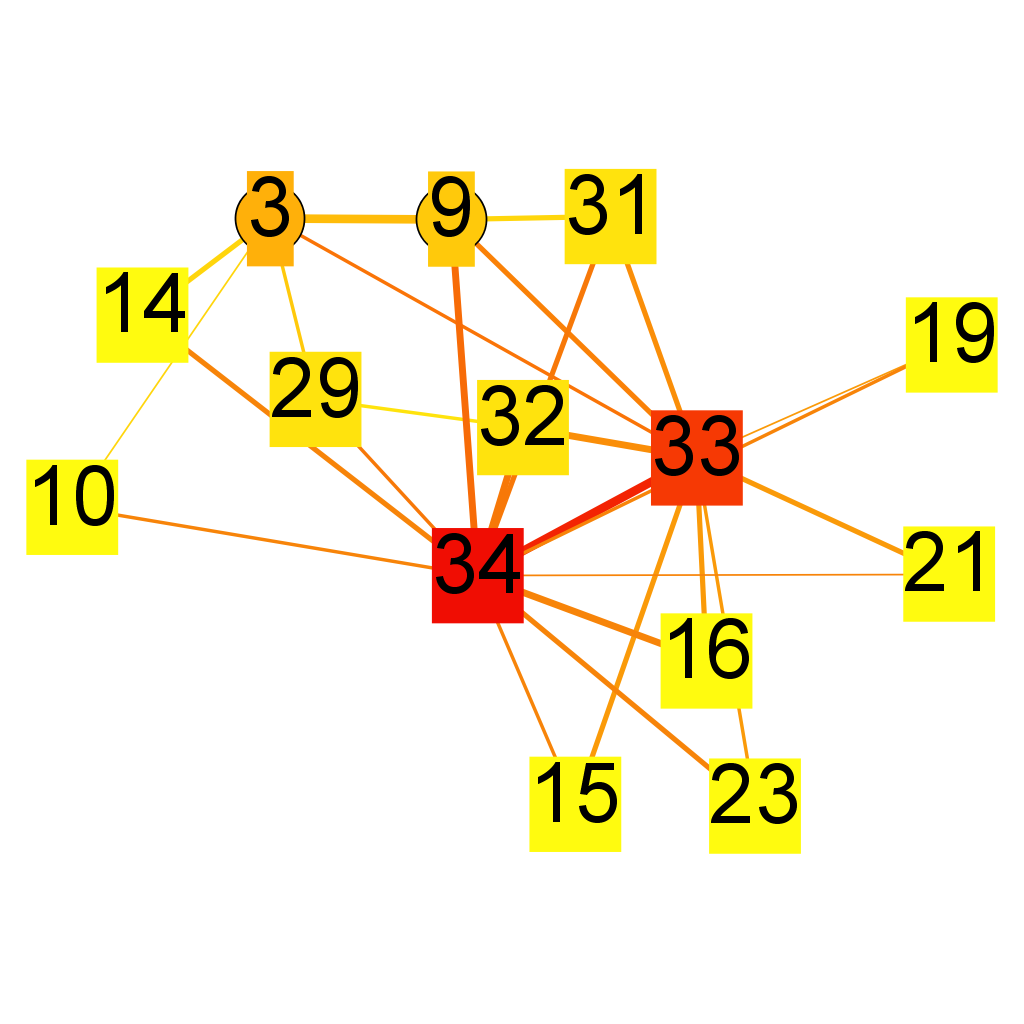
\includegraphics[width=1\textwidth]{4clubs/club2}
\caption{4-way Split Club 2}
\label{fig:4clubs2}
\end{minipage}
\end{figure}

\begin{figure}[H]
\centering
\begin{minipage}{.5\textwidth}
  \centering
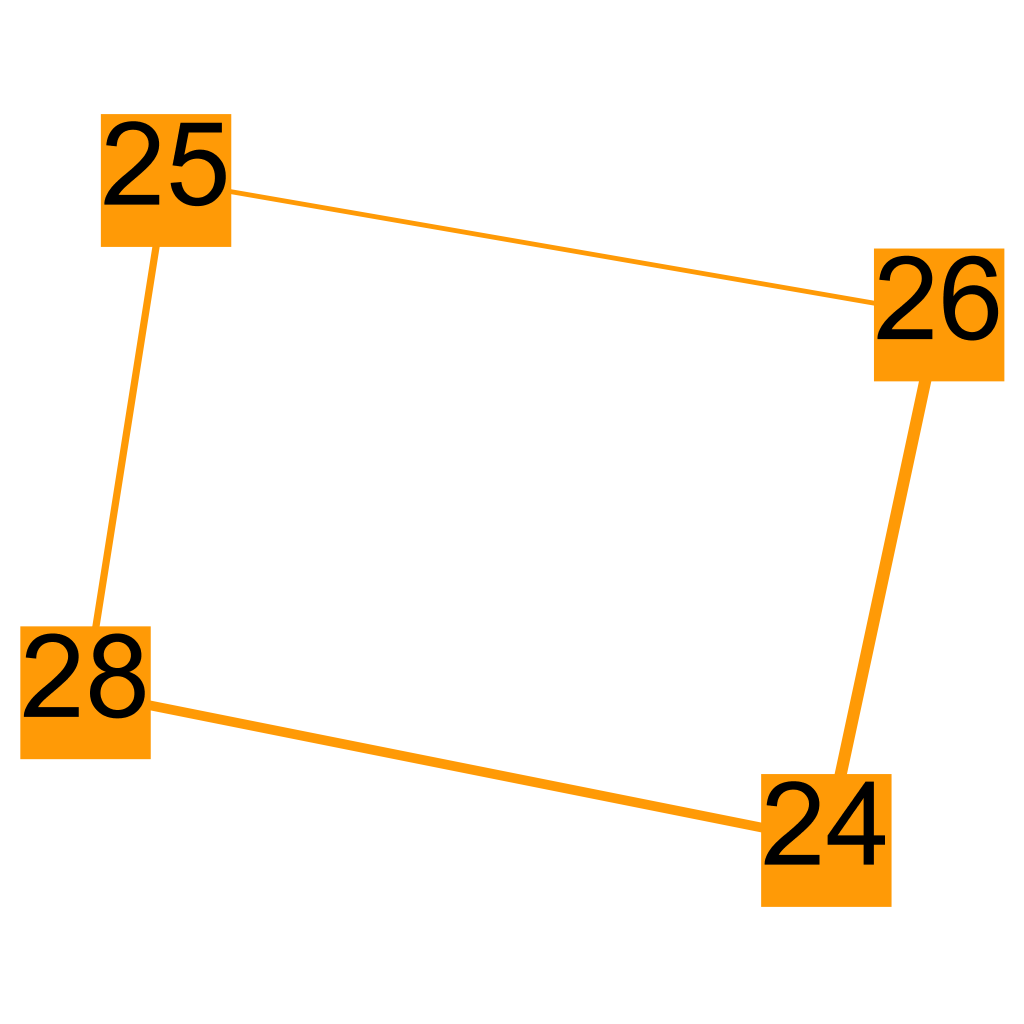
\includegraphics[width=1\textwidth]{4clubs/club3}
\caption{4-way Split Club 3}
\label{fig:4clubs3}
\end{minipage}%
\begin{minipage}{.5\textwidth}
  \centering
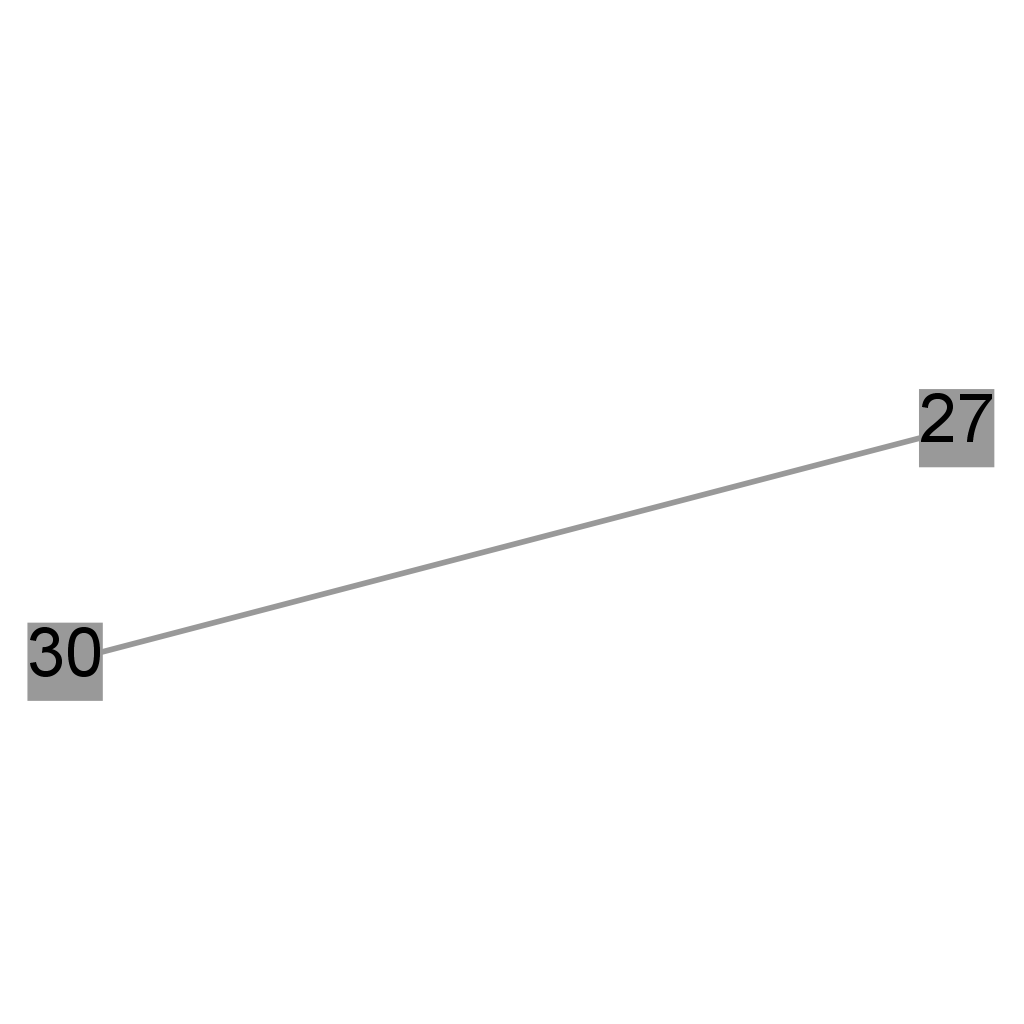
\includegraphics[width=1\textwidth]{4clubs/club4}
\caption{4-way Split Club 4}
\label{fig:4clubs4}
\end{minipage}
\end{figure}

\subsubsection{Five Clubs}
\begin{figure}[H]
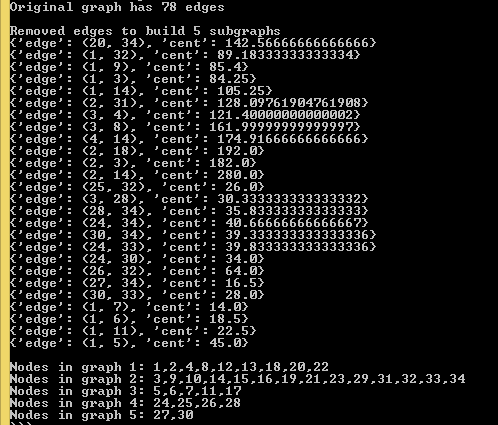
\includegraphics[width=1\textwidth]{5clubs/output}
\caption{Program Output 5 Clubs}
\label{fig:output5}
\end{figure}

\begin{figure}[H]
\centering
\begin{minipage}{.5\textwidth}
  \centering
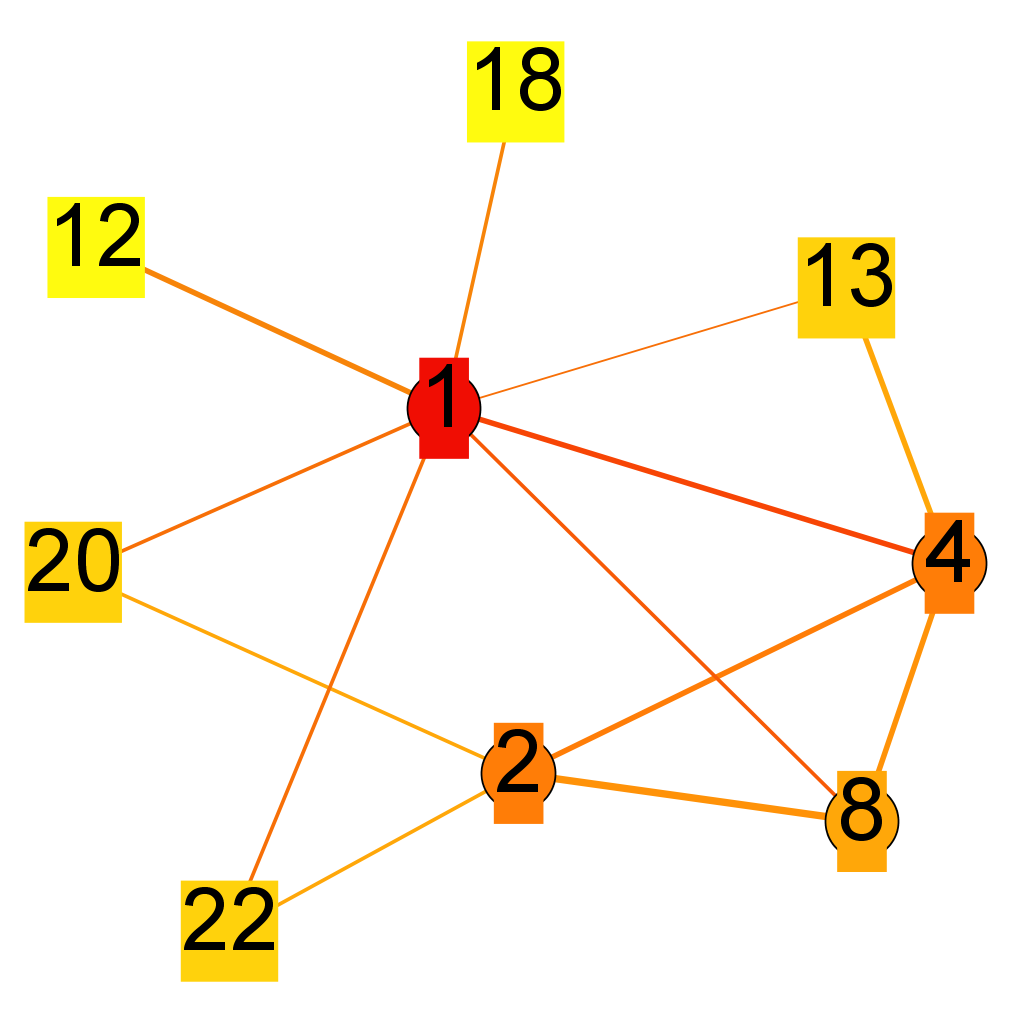
\includegraphics[width=1\textwidth]{5clubs/club1}
\caption{5-way Split Club 1}
\label{fig:5clubs1}
\end{minipage}%
\begin{minipage}{.5\textwidth}
  \centering
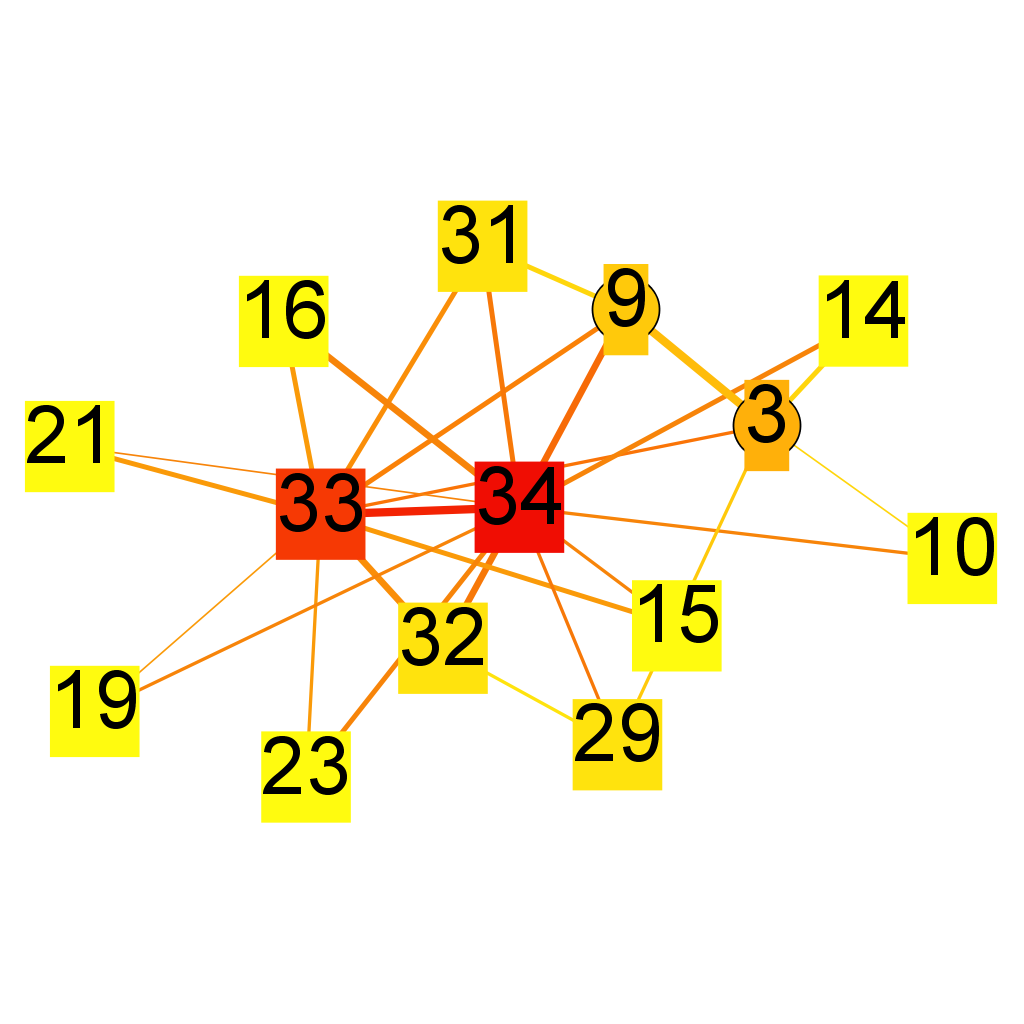
\includegraphics[width=1\textwidth]{5clubs/club2}
\caption{5-way Split Club 2}
\label{fig:5clubs2}
\end{minipage}
\end{figure}

\begin{figure}[H]
\centering
\begin{minipage}{.3\textwidth}
  \centering
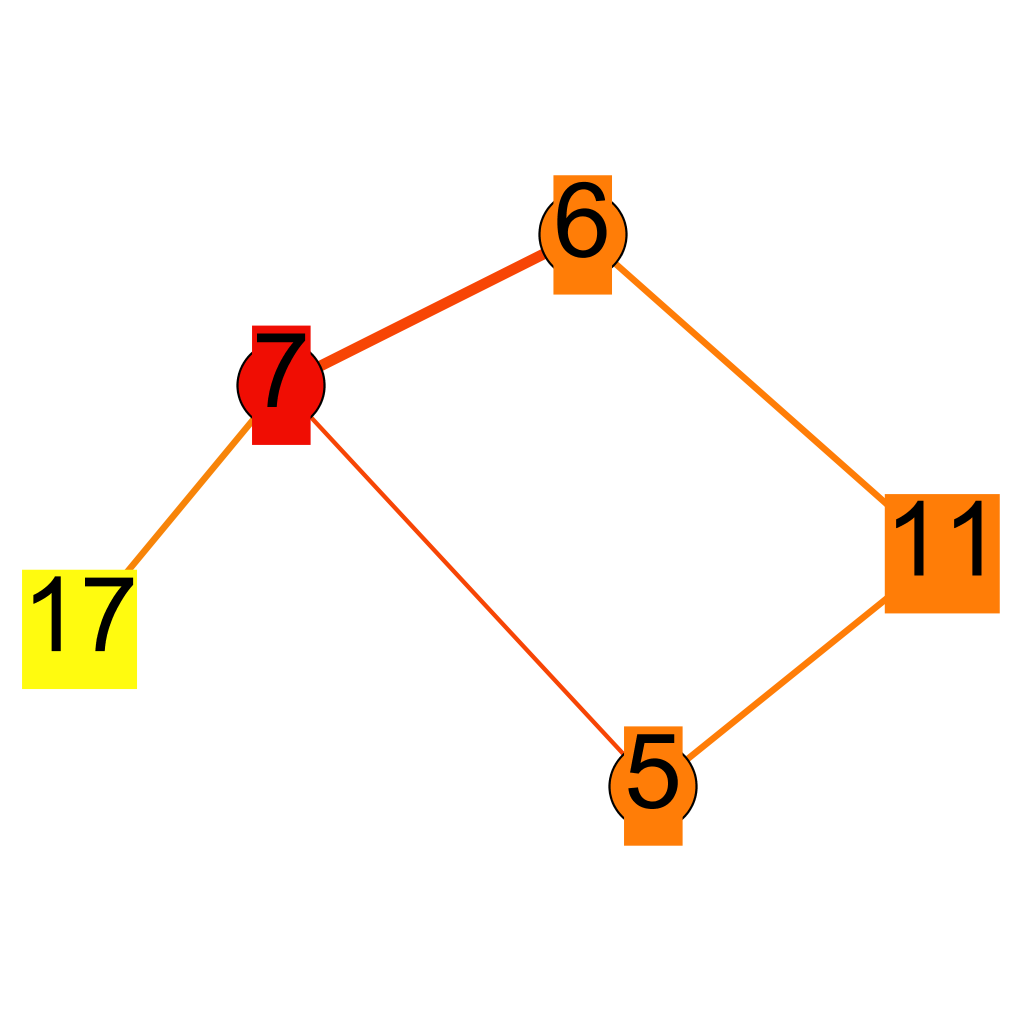
\includegraphics[width=1\textwidth]{5clubs/club3}
\caption{5-way Split Club 3}
\label{fig:5clubs3}
\end{minipage}%
\begin{minipage}{.4\textwidth}
  \centering
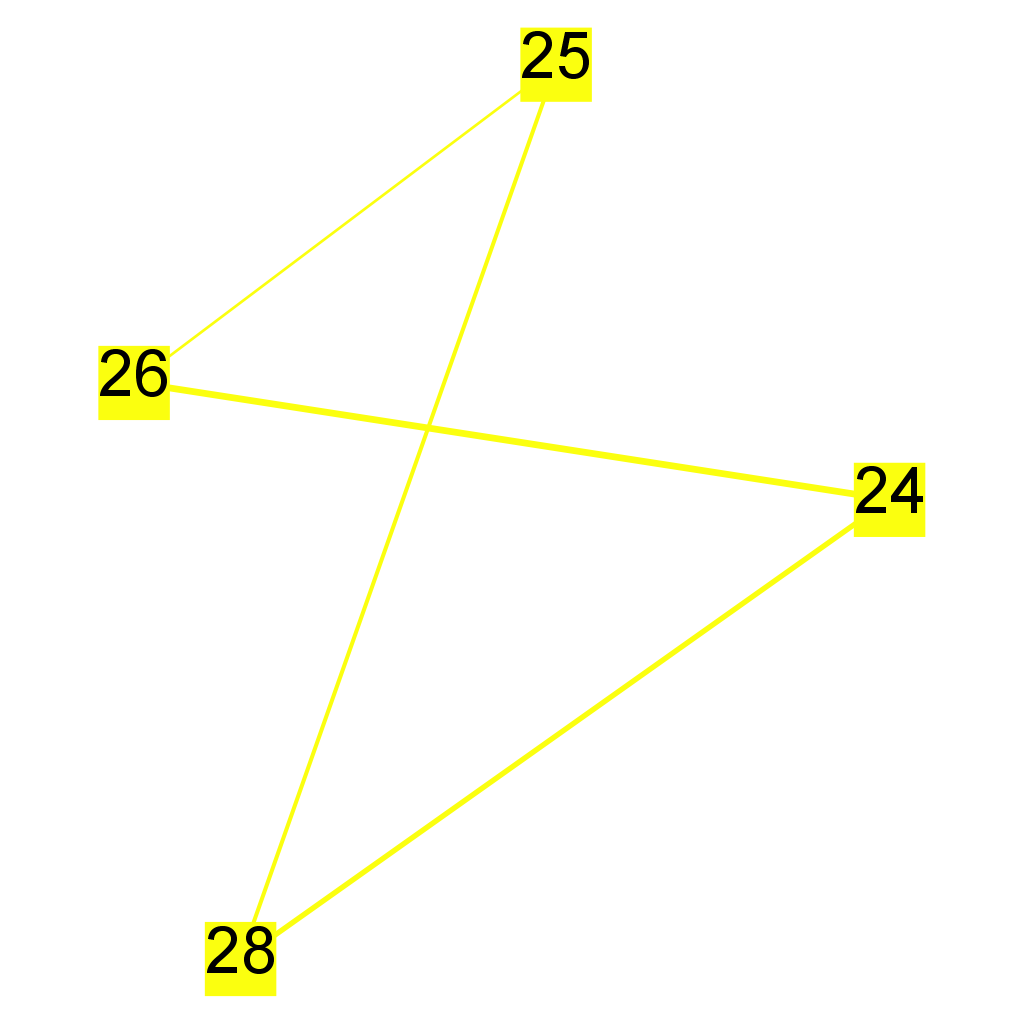
\includegraphics[width=1\textwidth]{5clubs/club4}
\caption{5-way Split Club 4}
\label{fig:5clubs4}
\end{minipage}%
\begin{minipage}{.25\textwidth}
  \centering
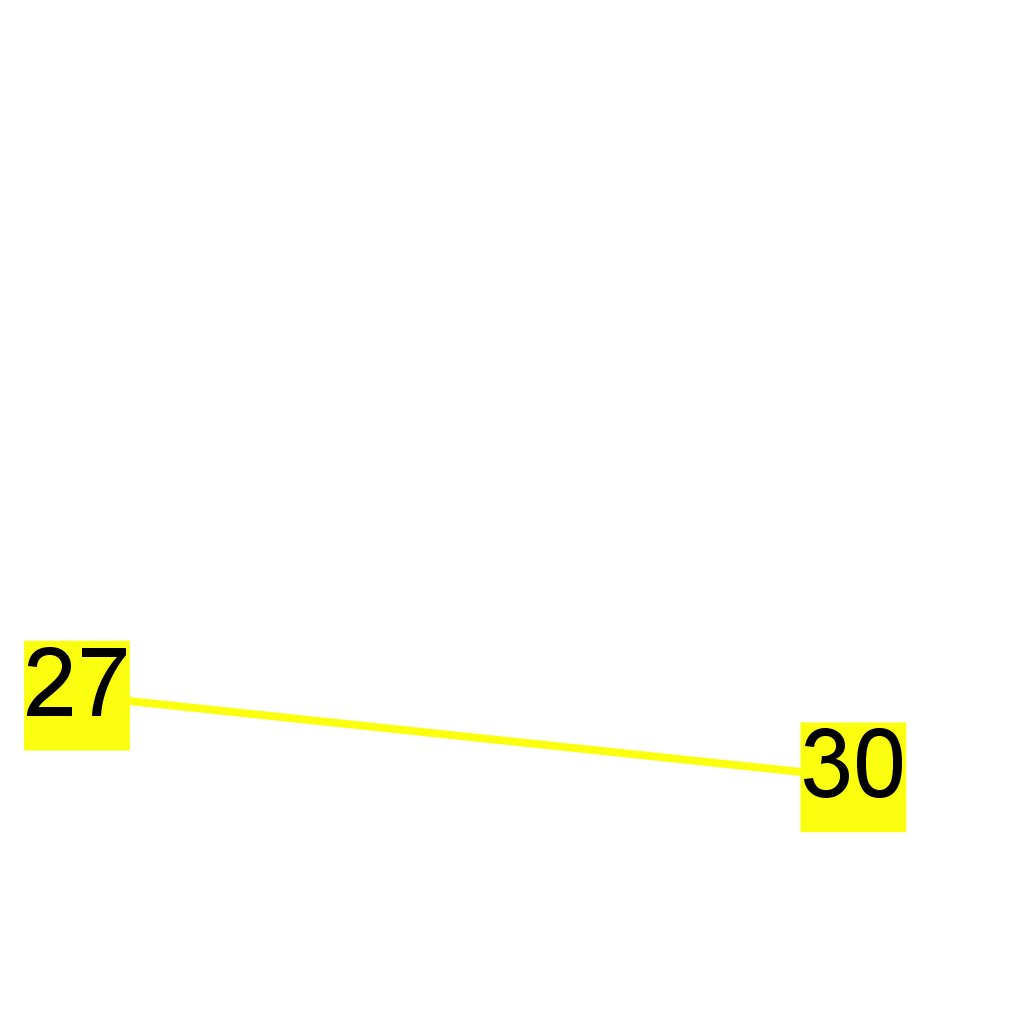
\includegraphics[width=1\textwidth]{5clubs/club5}
\caption{5-way Split Club 5}
\label{fig:3clubs3}
\end{minipage}
\end{figure}

\newpage

\bibliography{references}{}
\bibliographystyle{plain}
\end{document}